\documentclass[titlepage, a4paper]{article}

\usepackage[swedish]{babel}
\usepackage[utf8]{inputenc}
\usepackage{color}
\usepackage{graphicx}
\usepackage{etoolbox}
\usepackage{stringenc}
\usepackage{pdfescape}

% Sidformat
\usepackage{a4wide}

% Fixa Appendix-titlar
\usepackage[titletoc,title]{appendix}

% Bättre tabeller
\usepackage{tabularx}

% Bättre bildtexter
\usepackage[margin=10pt,font=small,labelfont=bf,labelsep=endash]{caption}

% Enkelt kommando som låter mig attgöra-markera text
\newcommand{\todo}[1] {\textbf{\textcolor{red}{#1}}}

% Nytt \paragraph låter oss ha onumrerade bitar
\makeatletter
\renewcommand\paragraph{\@startsection{paragraph}{4}{\z@}%
{-3.25ex\@plus -1ex \@minus -.2ex}%
{1.5ex \@plus .2ex}%
{\normalfont\normalsize\bfseries}}
\makeatother

\providecommand{\LIPSlogga}{../mall/logga2.png}
\providecommand{\LIPSdatum}{\today}

%% Headers och Footers
\usepackage{fancyhdr}
\pagestyle{fancy}
\lhead{\includegraphics[scale=0.4]{\LIPSlogga}}
\rhead{\ifdef{\LIPSutfardare}{Utfärdat av \LIPSutfardare \\\LIPSdatum}\LIPSdatum}
\lfoot{\LIPSkursnamn \\ \LIPSdokumenttyp}
\cfoot{\thepage}
\rfoot{ \LIPSprojektnamn}

%% Titelsida
\newcommand{\LIPSTitelsida}{%
{\ }\vspace{45mm}
\begin{center}
  \textbf{\Huge \LIPSdokument}
\end{center}
\begin{center}
{\Huge \LIPSprojektnamn}
\end{center}
\begin{center}
  {\Large Redaktör: \LIPSredaktor}
\end{center}
\begin{center}
  {\Large \textbf{Version \LIPSversion}}
\end{center}
\vfill
\begin{center}
  {\large Status}\\[1.5ex]
  \begin{tabular}{|*{3}{p{40mm}|}}
    \hline
    Granskad & \LIPSgranskare & \LIPSgranskatdatum \\
    \hline
    Godkänd & \LIPSgodkannare & \LIPSgodkantdatum \\
    \hline
  \end{tabular}
\end{center}
\newpage
}

% Projektidentitet
\newenvironment{LIPSprojektidentitet}{%
{\ }\vspace{45mm}
\begin{center}
  {\Large PROJEKTIDENTITET}\\[0.5ex]
  {\small
  \LIPSartaltermin,\\
  Linköpings Tekniska Högskola, IDA
  }
\end{center}
\begin{center}
  {\normalsize Gruppdeltagare}\\
  \begin{tabular}{|l|l|p{25mm}|l|}
    \hline
    \textbf{Namn} & \textbf{Ansvar} & \textbf{Telefon} & \textbf{E-post} \\
    \hline
}%
{%
    \hline
  \end{tabular}
\end{center}
\begin{center}
  {\small
    \ifdef{\LIPSgruppadress}{\textbf{E-postlista för hela gruppen}: \LIPSgruppadress\\}{}
    \ifdef{\LIPSgrupphemsida}{\textbf{Hemsida}: \LIPSgrupphemsida\\[1ex]}{}
    \ifdef{\LIPSkund}{\textbf{Kund}: \LIPSkund\\}{}
    \ifdef{\LIPSkundkontakt}{\textbf{Kontaktperson hos kund}: \LIPSkundkontakt\\}{}
    \ifdef{\LIPSkursansvarig}{\textbf{Kursansvarig}: \LIPSkursansvarig\\}{}
    \ifdef{\LIPShandledare}{\textbf{Handledare}: \LIPShandledare\\}{}
  }
\end{center}
\newpage
}
\newcommand{\LIPSgruppmedlem}[4]{\hline {#1} & {#2} & {#3} & {#4} \\}

%% Dokumenthistorik
\newenvironment{LIPSdokumenthistorik}{%
\begin{center}
  Dokumenthistorik\\[1ex]
  %\begin{small}
    \begin{tabular}{|l|l|p{60mm}|l|l|}
      \hline
      \textbf{Version} & \textbf{Datum} & \textbf{Utförda förändringar} & \textbf{Utförda av} & \textbf{Granskad} \\
      }%
    {%
			\hline
    \end{tabular}
  %\end{small}
\end{center}
}

\newcommand{\LIPSversionsinfo}[5]{\hline {#1} & {#2} & {#3} & {#4} & {#5} \\}

% Kravlistor
\newenvironment{LIPSkravlista}{
	\center
		\tabularx{\textwidth}{| p{1.2cm} | p{1.9cm} | X | c |}
			\hline
			\textbf{Krav} & \textbf{Förändring} & \textbf{Beskrivning} & \textbf{Prioritet} \\\hline
}
{
		\endtabularx
	\endcenter
}

\newcounter{LIPSkravnummer}
\addtocounter{LIPSkravnummer}{1}
\newcommand{\LIPSkrav}[4][Krav \arabic{LIPSkravnummer}]{{#1} & {#2} & {#3} & {#4} \stepcounter{LIPSkravnummer}\\\hline}


% Leveranskravlistor
\newenvironment{LIPSleveranskravlista}{
	\center
		\tabularx{\textwidth}{| p{1.2cm} | p{1.9cm} | X | X |}
			\hline
			\textbf{Krav} & \textbf{Förändring} & \textbf{Beskrivning} & \textbf{Deadline}\\\hline
}
{
		\endtabularx
	\endcenter
}

\newcounter{LIPSleveranskravnummer}
\addtocounter{LIPSleveranskravnummer}{1}
\newcommand{\LIPSleveranskrav}[4][Krav \arabic{LIPSkravnummer}]{{#1} & {#2} & {#3} & {#4} \stepcounter{LIPSkravnummer}\\\hline}


% Milstolps-lista
\newenvironment{LIPSmilstolpar}{
	\center
		\tabularx{\textwidth}{| p{1.2cm} | X | l |}
			\hline
			\textbf{Nr} & \textbf{Beskrivning} & \textbf{Datum} \\\hline
}
{
		\endtabularx
	\endcenter
}

\newcounter{LIPSstolpnummer}
\addtocounter{LIPSstolpnummer}{1}
%\newcommand{\LIPSmilstolpe}[3][Krav \arabic{LIPSstolpnummer}]{{#1} & {#2} & {#3} \stepcounter{LIPSstolpnummer}\\\hline}
\newcommand{\LIPSmilstolpe}[3]{{#1} & {#2} & {#3} \\\hline}

% Aktivitets-lista
\newenvironment{LIPSaktivitetslista}{
	\center
		\tabularx{\textwidth}{| p{0.3cm} | X | c | c | c |}
			\hline
			\textbf{Nr} & \textbf{Beskrivning} & \textbf{Beroende av} & \textbf{Timmar} & \textbf{datum} \\\hline
}
{
		\endtabularx
	\endcenter
}

\newcounter{LIPSaktivitetsnummer}
\addtocounter{LIPSaktivitetsnummer}{1}
% \newcommand{\LIPSaktivitet}[4][\arabic{LIPSstolpnummer}]{{#1} & {#2} & {#3} & {#4} \stepcounter{LIPSstolpnummer}\\\hline}
\newcommand{\LIPSaktivitet}[5]{{#1} & {#2} & {#3} & {#4} & {#5}\\\hline}

% Mall för mötesprotokoll
\newenvironment{projektmote}[2]{
  {\ }\vspace{5mm}

  \centerline{\textbf{\Huge #1}}
  \vspace{2mm}
  \centerline{\LARGE #2}
  \vspace{10mm}

  \begin{itemize}
}
{
  \end{itemize}
}

\newcounter{paragrafnummer}
\addtocounter{paragrafnummer}{1}
\newcommand{\paragraf}[1]{\item{\textsection \arabic{paragrafnummer}. {#1}}\addtocounter{paragrafnummer}{1}}

% Mall för Statusrapport
\newenvironment{statusrapport}{
  \center
    \tabularx{\textwidth}{| p{0.4cm} | X | X | p{14.5mm} | p{13.5mm} | p{16.5mm} | p{16.5mm} |}
    \hline
    \textbf{Nr} & \textbf{Aktivitet} & \textbf{Beroenden} & \textbf{Planerad tid} & \textbf{Nedlagd tid} & \textbf{Planerad klar} & \textbf{Beräknat klart} \\\hline
}
{
    \endtabularx
  \endcenter
}

\newcommand{\aktivitetstatus}[7]{{#1} & {#2} & {#3} & {#4} & {#5} & {#6} & {#7} \\\hline}	% Importera generella layout-strukturer

% Information nödvändig för generella layout-strukturer
\newcommand{\LIPSredaktor}{Sebastian Fast}
\newcommand{\LIPSversion}{1.0}
\newcommand{\LIPSdokument}{Uppbyggnad av stabila arkitekturer}
\newcommand{\LIPSdokumenttyp}{Kandidatrapport}
\newcommand{\LIPSgranskatdatum}{-}
\newcommand{\LIPSgranskare}{Sebastian Fast}
\newcommand{\LIPSgodkannare}{Andreas Runfalk}
\newcommand{\LIPSgodkantdatum}{-}
\newcommand{\LIPSkursnamn}{TDDD77}
\newcommand{\LIPSprojektnamn}{Prediktionsreglering}
\newcommand{\LIPSprojektgrupp}{Grupp 2}
%\newcommand{\LIPSgruppadress}{\todo{Ta bort}}
\newcommand{\LIPSartaltermin}{VT, 2015}
\newcommand{\LIPSgrupphemsida}{http://pum-2.ida.liu.se/}
\newcommand{\LIPSkund}{Saab}
\newcommand{\LIPSkundkontakt}{Daniel Simon}
\newcommand{\LIPSkursansvarig}{Kristian Sandahl}
\newcommand{\LIPShandledare}{Andreas Runfalk}

% Dokument-specifika paket
\usepackage{tabularx}
\usepackage{pdfpages}
\usepackage{tikz}
\usepackage{float}
\usepackage{graphicx}
\usepackage{algorithm}
\usepackage{algpseudocode}
\usepackage[round]{natbib}
\usepackage[nottoc]{tocbibind}
\usepackage{tcolorbox}
\usepackage{listings}
\usepackage{url}

\usetikzlibrary{shapes, arrows}

\pagenumbering{roman}
\renewcommand*{\thepage}{E-\roman{page}}

\DeclareGraphicsRule{.0.pdf}{pdf}{*}{}

\begin{document}

\LIPSTitelsida
\newpage
\tableofcontents	%Innehållsförteckning
\newpage
\pagenumbering{arabic}
\renewcommand*{\thepage}{E-\arabic{page}}
\section{Inledning}
Jag har gjort en filhanterar som visualiserar alla filer och mappar i 3D med hjälp av OpenGL. Inspirationen till detta projekt var bland annat FSN (File System Navigator) som gjordes av SGI för IRIX systemen och FSV(File System Visualizer) som är en remake av FSN på Linux, se figur~\ref{fig:fsn}. En annan inspiration var det lite modernare TDFSB som även visar upp bilder och filmer i 3D världen, se figur~\ref{fig:tdfsb}. 

\begin{center}
\begin{figure}[H]
    \centering
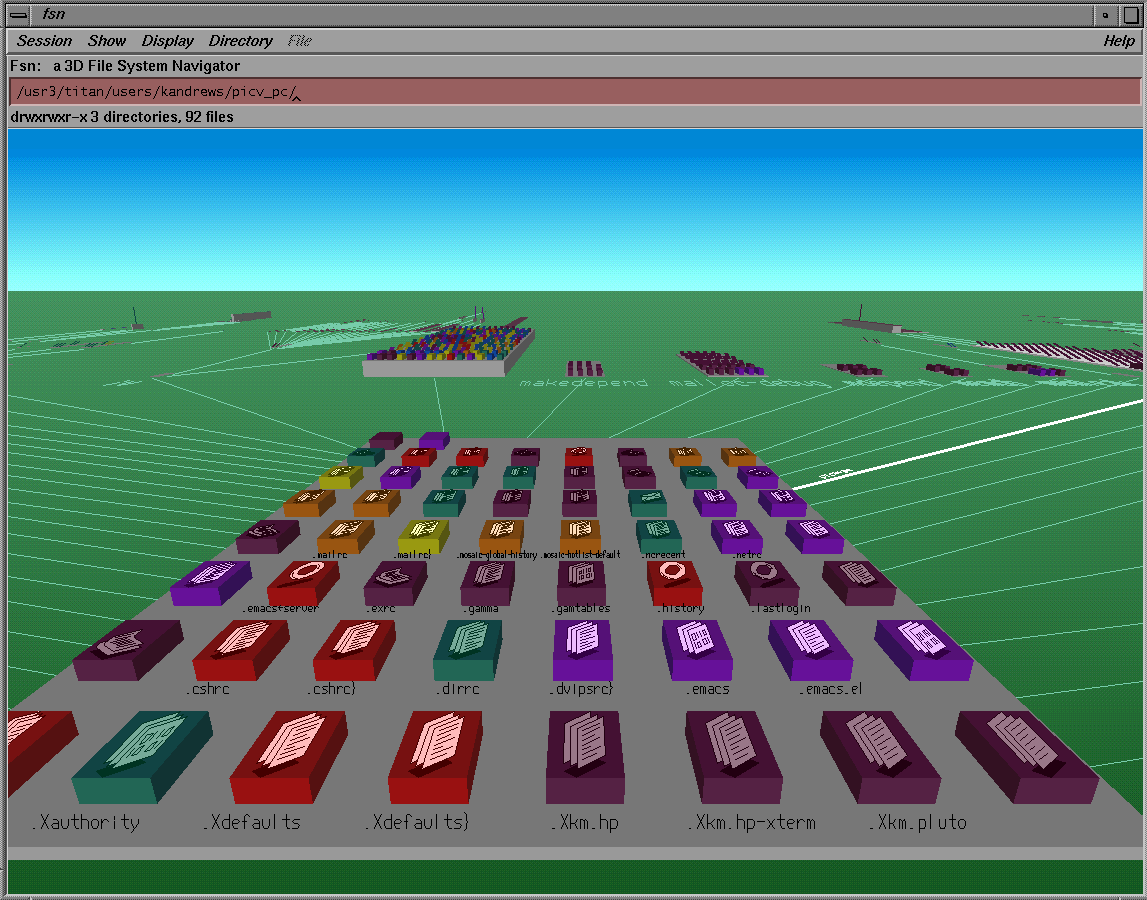
\includegraphics[width=8cm]{../grafik/fsn1.png}
\caption{FSN.}
\label{fig:fsn}
\end{figure}
\end{center}

\begin{center}
\begin{figure}[H]
    \centering
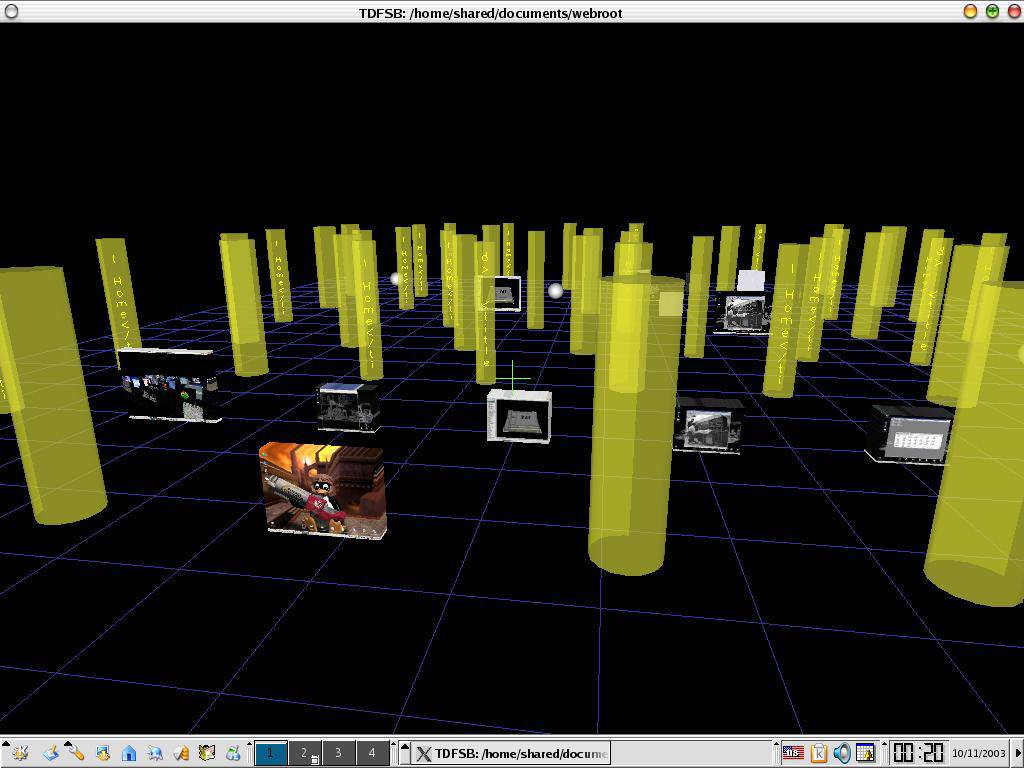
\includegraphics[width=8cm]{../grafik/tdfsb.jpg}
\caption{TDFSB.}
\label{fig:tdfsb}
\end{figure}
\end{center}

De ursprungliga obligatoriska kraven för produkten var följande:
\begin{LIPSkravlista}
\LIPSkrav{Original}{Alla filer ska representeras av block med någon textur på, är det en bild så ska bilden användas som textur}{1}

\LIPSkrav{Original}{Alla mappar ska representeras av block med någon textur}{1}
\LIPSkrav{Original}{Alla mappar och filer i en mapp ska vara placerade på en platta med en textur}{1}
\LIPSkrav{Original}{Ljussättningen ska ske med en Phong-shader}{1}
\LIPSkrav{Original}{Alla block ska ha skuggor}{1}
\LIPSkrav{Original}{Navigeringen ska vara first person där piltangenterna styr x och z koordinaterna och musen styr kameren i ett sfäriskt koordinatsystem}{1}
\LIPSkrav{Original}{Man ska inte kunna gå igenom filerna(collisions detection)}{1}
\LIPSkrav{Original}{Du ska kunna gå in i en mapp så transporteras du till den nya mappen)}{1}
\LIPSkrav{Original}{Du ska kunna klicka på en fil/mapp och få upp alla möjliga alternativ såsom radera, öppna...)}{1}
\LIPSkrav{Original}{Om du raderar en fil ska övriga filer ordna sig så det inte är några luckor någonstans}{1}
\LIPSkrav{Original}{Skydome ska finnas}{1}
\LIPSkrav{Original}{Endast Linux kommer stödjas}{1}
\end{LIPSkravlista}


och de ej obligatoriska kraven var följande:
\begin{LIPSkravlista}
\LIPSkrav{Original}{Du ska kunna få upp en terminal i filhanteraren}{2}
\LIPSkrav{Original}{Du ska kunna klicka på en mapp och sedan få upp en portal som du kan se in i mappen genom}{2}
\LIPSkrav{Original}{När du raderar en fil ska den explodera}{2}
\LIPSkrav{Original}{Innehåller en mapp många filer/mappar ska frustum culling användas för att minimera beräkningar}{2}
\LIPSkrav{Original}{Mapparnas texturer ska vara den ikon filen som operativsystemet använder med transparens, då ska renderingsordningen och vara korrekt}{2}
\end{LIPSkravlista}
Under projektets gång gick de obligatoriska kraven igenom en modifikation på grund av att projektet tog längre tid än vad jag trodde samt att en del inte riktigt passade in. Krav 5 togs bort på grund av tidsbrist, krav 6 gjordes om så att användaren bara navigerade i XZ planet då detta passade mycket bättre samt en del förenklingar kunde göras. Krav 9 togs bort då en terminal ansågs vara mycket enklare att implementera så all modifikation av filsystemet görs via den. Inga av de ej obligatorska kraven uppfylldes på grund av tidsbrist. I figur~\ref{fig:tmbtrf} kan man se resultatet. 
\begin{center}
\begin{figure}[H]
    \centering
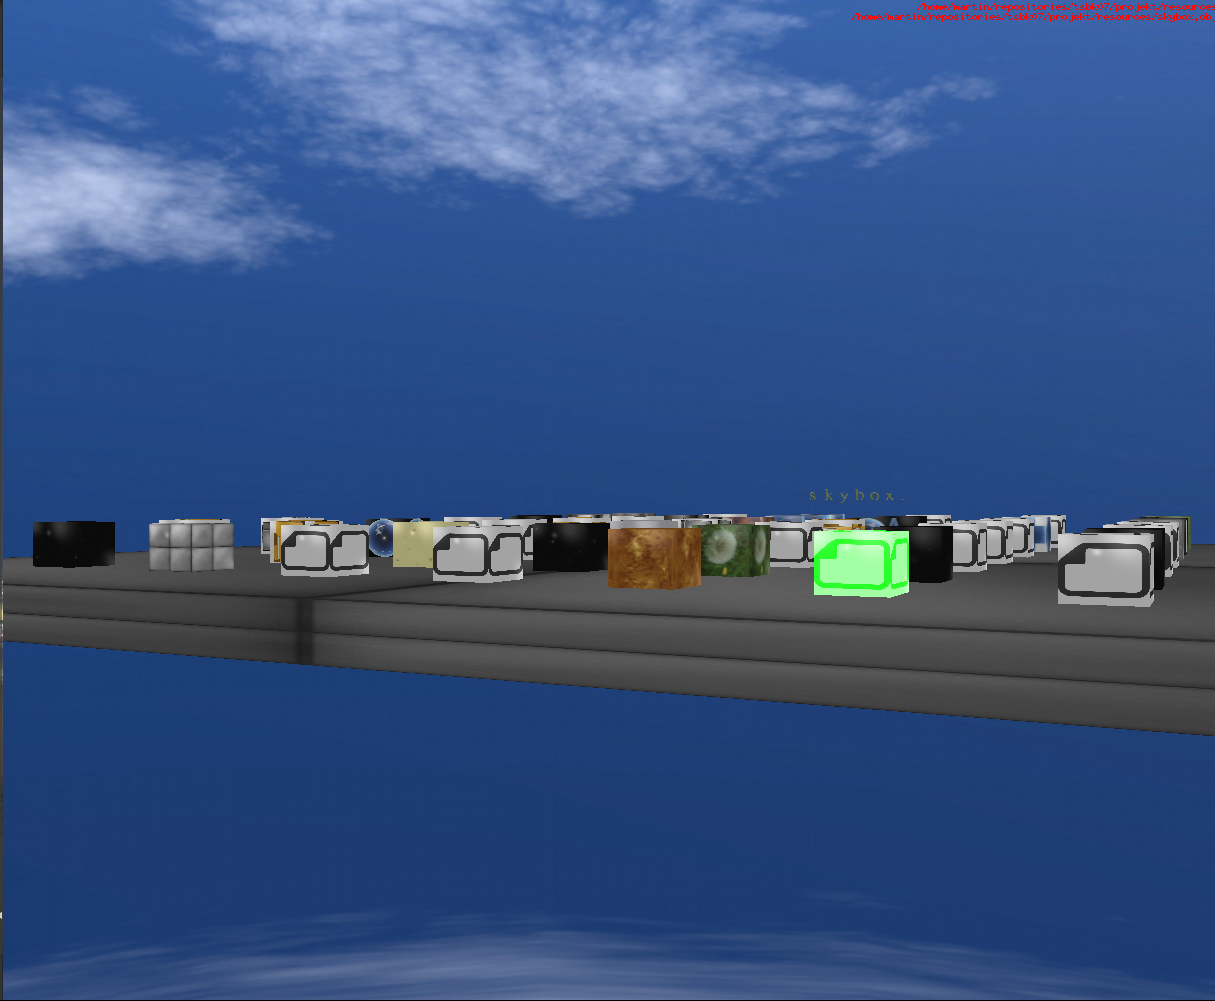
\includegraphics[width=8cm]{../grafik/tmbtrf.png}
\caption{TMBTRF.}
\label{fig:tmbtrf}
\end{figure}
\end{center}

\section{Bakgrund}
Det svåraste problemet jag hade innan jag började med projeketet var att på ett effektivt sätt interagera med datorns filsystem. Detta löstes rätt enkelt när jag upptäckte Boost::Filesystem. Detta bibliotek är inte speciellt använt så det finns inte så mycket hjälp att hitta på forum men dokumentation för det är väldigt bra så när jag väl kom in i det så fungera det väldigt bra. Funktioner såsom att byta namn och radera filer fanns redan implementerade så detta underlättade mycket.
\\
\\
Ett annat problem som var svårare än vad jag trodde var att visa filnamn i en 3D miljö. Den enklaste lösning skulle varit att använda något bibliotek för att generera texturer med en font till exempel FreeType. Jag försökte detta och jag kommer inte ihåg varför men jag fick det inte att fungera. För att få detta snyggt så skulle texturerna behöva vara transparenta så jag skulle behöva ta hänsynt till ordningen som alla objekt renderas. Min lösning på problemet var att generera .obj filer för alla tänkbara bokstäver och tecken som kan förekomma i ett filnamn. Jag valde alla bokstäver a-z och A-Z, alla siffror samt tecknen . - \_. Detta gjordes med ett python script i cad-programmet FreeCad. För att minimera inläsningstiden så läses alla dessa modeller in vid starten av programmet och återanvänds hela tiden. För att undvika problem som kan uppkomma vid långa filnamn som sträcker sig över hela miljön så visas bara de 7 första tecknen i filnamnet.
\\
\\
Anledningen till att C++ valdes var mest för dess datastrukturer såsom Vector, Map och string. Allting som kan göras i C++ kan självklart göras i C men där så är allting klart. Detta gjorde så att jag kunde göra en väldigt allmän klass som representerar alla objekt i 3D världen. Programmet arbetar också mycket med strängar och då är String väldigt mycket smidigare än en char array.
\\
\\
Ett problem som upptäcktes senare var att när man går in i en mapp som innehåller många filer, speciellt bilder, så tar det rätt lång tid innan hela världen har genererats. Detta skulle kunna lösas genom att ha en separat tråd som förbereder alla undermappar i den nuvarande mappen. Detta har dock inte implementeras men skulle jag fortsätta utveckla TMBTRF så skulle detta vara ett av de första problemen jag skulle lösa. 

\section{Teori}
I boken ''Software Product Quality Control'' \citep{SPQC} nämns ett antal definitioner som förtydligar vad kvalitetssäkring innebär, dessa syns nedan.  

\begin{itemize}
  \item ''Quality assurance: a planned and systematic pattern of all actions necessary to provide adequate confidence that an item or product conforms to established technical requirements.'' \citep[p.19]{SPQC} 
  \item ''Constructive quality assurance: All means to be used in constructing a product in a way so it meets its quality requirements.'' \citep[p.19]{SPQC} 
  \item ''Analyctical quality assurance: All means of analysing the state of the quality of a product.'' \citep[p.19]{SPQC} 
\end{itemize}
\noindent Kvalitetssäkring innebär följaktligen att man som leverantör av en produkt eller tjänst ska se till att de uppfyller de krav som har satts upp i en eventuell kravspecifikation. Det är dessa krav som sätter standarden för vad som är rätt nivå gällande kvalité. Under arbetsgången måste man analysera om man är på väg att uppfylla kraven eller inte, i sådana fall måste detta åtgärdas omedelbart.
\newline
\newline
Med detta sagt finns det flera steg i ett projekt att kvalitetssäkra. Ett effektivt sätt att göra detta på är genom att följa Shewhart cykeln, det vill säga planera, göra, studera och agera (PGSA) \citep{PDCA}. Shewhart cykeln är en iterativ fyra stegs metod, se figur \ref{fig:shewcycle}. Metoden är utvecklad av William Edwards Deming. Namnet ''Shewhart'' kommer från en av Demings kollegor \citep[p.~88]{Deming}. 
\begin{figure}[h]
\centerline{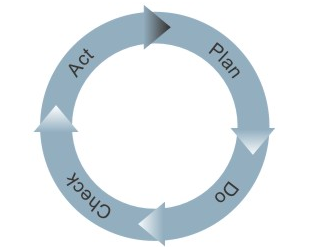
\includegraphics[scale=0.5]{ruben-tex/graphic/shewhartcycle}}
\caption{Shewhart cykeln \citep{Mindtools}}
\label{fig:shewcycle}
\end{figure}
\begin{enumerate}
  \item Planera. I detta skede ska målet fastställas, det vill säga sätta upp de krav som behövs för att kunden skall bli nöjd. Genom att göra detta är det tydligt om vad som skall göras och en överenskommelse finns mellan kund och leverantör. 
  \item Göra. När man konstaterat vad som behöver göras för att kunden skall bli nöjd är det dags att implementera ett sätt att arbeta och fullfölja processen.
  \item Studera. Efter att ha följt processen under en viss period är det dags att utvärdera om processen man har följt kommer leda till att man uppfyller de målen man har fastställt i planeringsfasen.
  \item Agera. Om man under studeringsfasen upptäcker att processen man följer inte kommer leda till att man uppfyller de krav som kund och leverantör var överens om måste detta åtgärdas omedelbart genom att planera om arbetsprocessen eller i viss mån diskutera kraven med kunden. Om processen som följs kommer uppfylla de krav som har satts upp kan man fortsätta med iterationerna av Shewhart cykeln precis som innan.
\end{enumerate}
\begin{figure}[h]
\centerline{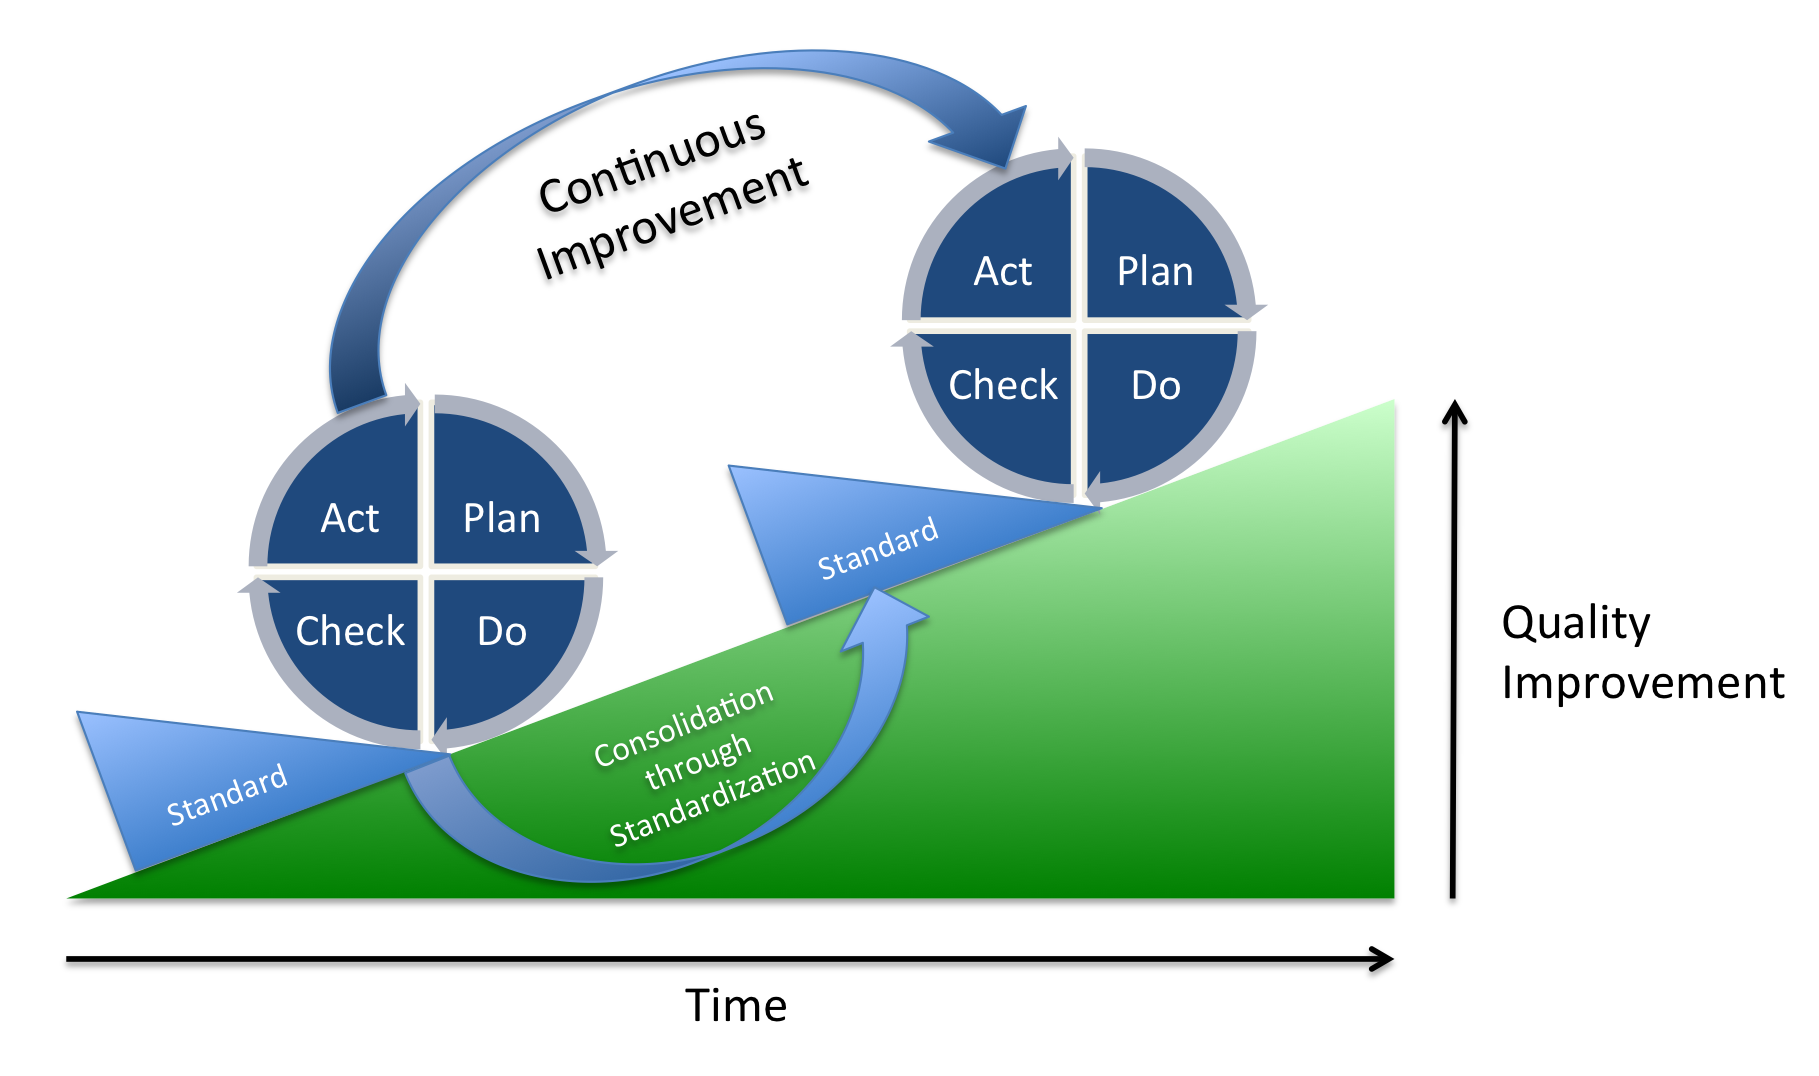
\includegraphics[scale=0.15]{ruben-tex/graphic/PDCA_Process}}
\caption{PDCA process \citep{Vietze}}
\label{fig:pdcaprocess}
\end{figure}
\noindent Genom att följa Shewhart cykeln under ett projekt kan man iterativt förbättra sin arbetsprocess och genom detta öka kvaliteten av den produkt man utvecklar, se figur \ref{fig:pdcaprocess}.
\newline
\newline
När det väl är dags för överlämning av en produkt eller tjänst är det bra att göra en kravinspektion innan. En kravinspektion enligt IEEE standarden för ''Software reviews'' syns nedan.

\begin{tcolorbox}[boxrule=1pt,leftrule=5pt,arc=0pt,auto outer arc]
\textbf{''}A process or meeting during which a software product is examined by a project personnel, managers, users, customers, user representatives, or other interested parties for comment or approval\textbf{''} \citep{SFSR}
\end{tcolorbox}

\noindent
Det man vill få gjort med en kravinspektion är alltså att produkten eller tjänsten som har tagits fram ska utvärderas av berörda parter så att den uppfyller de krav som har fastställts i ett tidigare skede för ett godkännande. En kravinspektion kan se ut som sådan \citep{Sandahl}:
\begin{enumerate}
\item{Tillträde.}
\item{Planering och översikt. Under detta steg sker en planering över hur inspektionen ska gå till och en översikt av produkten ges.}
\item{Individuell granskning. De berörda parterna granskar produkten eller tjänsten.}
\item{Möte. Efter granskningen görs en lista av alla de defekter som kan ha hittats.}
\item{Ändringar och uppföljning. I detta skede åtgärdar man de defekter som stöttes på och normalt brukar verifiera detta.}
\item{Utträde.}
\end{enumerate}

\subsection{Sammanfattning}
Sammanfattningsvis kan man konstatera att ett återkommande tema för att ta fram en högkvalitativ produkt eller tjänst är att planera, utföra och granska, för att sedan upprepa proceduren under projektets gång. Detta är dock bara en teoretisk tillämpning och verkligheten kan se annorlunda ut.

\section{Metod}
	För att ta reda på all information som behövs har ett flertal böcker blickats igenom. Ingen av dem har läst till 100\%, utan endast de intressanta delarna har läst med mer nogrannhet. För att verifiera att det som lästs stämmer har vissa delar testats i praktiken, i detta fall på projketet. Till exempel så har enhetstester körts på matris bibliotekts funktioner såsom matrisaddition, sytemtester och modultester har körts på den kvadratiska problem-lösaren och acceptanstester har körts på alla delar i projektet för att se till att alla krav är uppfyllda. Mer om detta kan läsas i resultat.
	
\subsection{Enhetstest}
	I ''Software Unit Testing'' \citep{ivv} definierar ett enhetstest som ett test på den minsta möjliga samlingen kod som fortfarande går att testa nyttofullt, alltså att koden är tillräckligt stor för att fel ska kunna uppstå. Dessa test är bra då de är riktade mot en så liten portion med kod och i och med detta sällan missar buggar och fel. Det som kan vara krångligt med enhetstest är att just hitta dessa minsta samlingarna med kod, speciellt om det är en extern part (en annan programmerare) som ska skapa och utföra testen. I och med att man kör enhetstester på så små delar av kod har de i teorin en tendens till att bli väldigt många om man ska täcka tillräckligt stor funktionalitet. Detta är dock oftast inget problem i praktiken eftersom många små funktioner ofta är triviala och har ytterst få uppgifter. Då behöver inte så många test skrivas, om ens ett enda.
\subsection{Modultest}	
	Det finns flera olika definitioner av vad en modul är, och i och med det blir det då svårt att definiera vad ett modultest är. I ''The Art of Software Testing'' definierar de att moduler och enheter är samma sak men jag har valt att istället gå efter Kristian Sandahls definiton. Han definierar att ett modultest är ett integrationtest utav två eller fler enheter. Det går ut på att man kombinerar ett antal enheter och sedan testar dem tillsammans. Testen i sig kan var väldigt lika enhetstest men täcker nu en mer komplex funktionalitet. Precis som enheter kan moduler vara svåra att definiera. Om allt för många enheter förs samman och modulen får mer funktionalitet kanske den till slut kan klassas som ett system, och då förlorar modultestningen sitt syfte. Om man har ett så litet projekt som detta så är moduldefinitionen ofta inte så svår, eftersom både komplexiteten och utvecklingsmöjligheterna är begränsade. Det är kritiskt vid dessa test att underliggande funktioner redan är testade. Om inte, kan i stort sett inga slutsatser, angående vad som är fel, dras när ett test misslyckas.
\subsection{Systemtest}	
	Ett systemtest är precis som modultest ett integrationstest, men nu utav ett antal moduler istället. Enligt ''The Art of Software Testing'' inriktar sig testet nu också vanligtvis på hela produkten som har utvecklats, för att se om funktionalitetskraven är uppfyllda. Detta för att säkerställa dess funktionalitet och för att hitta fel som uppstått vid kommunikation mellan moduler. Exempel på systemtest i vårt projekt är test av lösaren. Anledningen till att lösaren ses som ett eget system och inte är ihopbakad med GUI:t är att den ska kunna fungera separat. Givetvis är de båda ihopbakade också ett system, som också kräver systemtest.	
\subsection{Acceptanstest}	
	Ett acceptanstest är ett test som har målet att testa om programmet är acceptabelt. Med det menas att testen validerar ifall programmet uppfyller alla krav som ställs på det, och nu inte endast funktionalitetskraven. I vårt projekt är det huvudsakligen prestandan som behöver acceptanstestas. Då det prestandakrav produkten hade var relativt vagt ("Produkten ska ha likvärdig prestanda med Gurobi"), och att kravet sedan förhandlades bort, gjorde att testen inte hade så stor prioritet. Men för att få någon vetskap om produktens hastighet och för att garantera att kunden blir nöjd krävs ändå någon form utav test.
\subsection{Övrigt}	
	I projektet har även ett byggsystem använts, som smidigt kompilerat all kod automatiskt. Systemet har därefter även kört alla tester som skapats genom projektet.
	Med hjälp av byggsystemet och Kontinuerlig Integration har all kod då kunnat testas direkt när någon har skrivit ny kod och därav har det gått att se när och var feluppstått. Och eftersom systemet även har kört alla gamla test har koden säkerställts med att alla andra funktioner, de som inte har rörts, också fortfarande fungerar.
\section{Resultat}	
	Följande del beskriver hur arbetet med efterforskningen gick samt hur testen utfördes.
	\subsection{Efterforskning}
	Det finns otroligt mycket information om mjukvarutestning men samtidigt är ämnet ganska vagt då testning beror så mycket på just vad som ska testas. I vårt projekt visade det sig att ''Black Box''-testning var den metod som överlägset lämpade sig bäst. ''Black Box'' går ut på att man sätter en ''svart låda'' över det som ska testas, så att man endast kan se in- och utdatan. Sedan tittar man på utdata och ser ifall den är den förväntade. ''Black Box'' anses bra i detta projekt eftersom hela Quadopt är uppbyggd utav många små funktioner och resultateten som de ska ge tillbaka är oftast kända på förhand. Ett exempel på detta är matrisaritmetiken där resultatet, av till exempel en multiplikation, går att räkna ut ganska enkelt på papper. Enligt ''The Art of Software Testing'' ska dessa test utgå ifrån kravspecifikationen och andra dokument som beskriver vad produkten ska ha för funktionalitet. Boken beskriver också ''Black Box'' som en utmattande testteknik. Med det menar de att man borde testa alla möjliga indata till den svarta lådan och se så att svaren stämmer. Detta är precis som det står i boken i praktiken omöjligt. Speciellt i vårt projekt där det enda som begränsar antalet olika sätt en matris, bestående utav tal, kan se ut på är datorns minne. \newline
I projektet fanns dock ofta behovet av se en funktions lösningsgång, och då är ''Black Box'' en väldigt dålig metod. En metod som då lämpar sig bättre är ''White Box'' testning, som innebär att man tittar på den interna strukturen i en funktion. Därefter kan man se, efter vald indata, om lösningsgången är den väntade. I ''The Art of Software Testing'' står det att även denna metod kan problematisk då antalet lösningsgångar kan vara väldigt många. För att se om det ens är rimligt att utföra dessa test kan man se på funktionens cyklomatiska komplexitet. Cyklomatisk komplexitet innebär att man gör en graf över funktionen där de möjliga stadierna i lösningsgången är noder, och de möjliga lösningsvägarna är bågar. I ''Structured testing'' \citep{structest} står det att om denna komplexitet är för stor ökar antalet fel som programmeraren gjort väldigt fort, och samtidigt blir det i stort sett omöjligt att utföra några ''White Box''-test då fel kan uppstå på så många ställen. \\ 	
För att säkerställa projektets krav behövdes bara en testmetod till, och det var en metod för att mäta prestanda. Den som valdes var ''Load testing'' som innebär att man belastar programmet med mycket data och ser hur bra det fungerar. I projektets fall gavs lösaren många problem och tittade på hur fort det gick i förhållande till andra lösare. \newline	
Det skulle kunnat varit så att GUI:t hade haft högre prioritet än vad det hade. I det fallet hade olika typer av UX- och användartest varit nödvändiga för att kvalitetssäkra produkten. Men eftersom GUI:t beställdes utifrån kundens personliga behov, var det tydligt definierat redan från början att det var av låg prioritet. 
	
	\subsection{Praktik}
	Som beskrivet tidigare finns det i stort sett oändligt många kombinationer av in- och utdata.	För att då kunna utföra ''Black Box''-testerna behövdes antalet testfall reduceras. Detta åstadkoms genom att ha möten med kunden som klargjorde att indata till programmet alltid skulle vara giltig. Det reducerade antal testfall enormt mycket, men som beskrivet i resultatet av efterforskningen finns det även väldigt mycket giltig indata. Exempelvis för matrisaritmetiken. Dessa test gick också att reducera genom att de flesta operationer är triviala och endast kräver numeriska test såsom nolldivision och flyttalsfel. Genom att även utnyttja ''White Box''-tekniken gick det att utforma olika ''Black Box''-test som tog olika vägar genom koden och på så sätt bara skapa ett test för varje väg. Denna teknik utnyttjades endast på mindre funktioner såsom moduler för att antalet olika fall skulle begränsas till något som var rimligt. \newline
	För lösaren gick det att applicera samma metod, eftersom dess funktionalitet bygger mycket på underliggande funktioner. Det som skilde sig gentemot småfunktionerna var att nu behandlades oftast rader eller kolumner i matriser istället för enskilda element. Detta ledde till att de flesta test kontrollerade på kanterna utav det tillåtna området. Alltså kunde ett test vara att försöka hämta ut en radvektor på rad -1 ur en matris, vilket skulle vara ogiltigt.\newline
Vid granskning av testresultat från Git, Travis (verktyg för Kontinuerlig integration) och gruppmedlemmar visade det sig att majoriteten fel av bestod utav två typer: ''Assertion''s som misslyckats och ''Segmentation fault''. En ''Assertion'' är ett test inuti koden som avbryter exekveringen om testet inte går bra. ''Segmentation fault'' är ett programmeringsfel som resulterat i en ogiltig läsning eller skrivning till minnet. Felen som uppstod var väldigt utspridda och olika. Det som de flesta hade gemensamt var dock att de låg på en låg nivå, alltså i bottenfunktionerna. \newline	
	För att testa algoritmens hastighet stötte gruppen på oväntade problem, lösarna var för snabba.	Då varje testkörning tog 0.00 sekunder för alla lösarna förutom MATLAB behövdes testen köras många gånger för att se en tydlig skillnad. Anledningen till att MATLAB är långsammare är för att den är oerhört generell men förmodligen inte gjorts med fokus på att vara snabb. Gurobi är snabb eftersom dess enda uppgift är att lösa sådana här problem och har arbetats på under lång tid. Vår algoritm är snabb eftersom den inte är generell, alltså bryr vi oss inte om vissa specialfall som vi aldrig kommer stöta på. \newline
	För att då testa deras prestanda fick lösarna lösa olika optimeringsproblem många gånger, ofta upp emot 1000 gånger, för att kunna skilja deras egentliga hastighet. Att köra testen på vår lösare och i MATLAB var enkelt då vi hade funktionalitet för att konvertera matriser från MATLABs definition till vår, och vice versa. Däremot så var det krångligare i gurobi eftersom tiden som var allokerad för utbildning av programmet var begränsad. Det tvingade gruppen till att mata in problemet på ekvationsform vilket gjorde att gruppmedlemmarna var tvungna att köra endast små tester. Redan vid problem med fler än 10 bivillkor skulle det ta väldigt lång tid att konvertera och mata in problemet. \newline
	
	
	\subsection{Enhetstester}
	Under projektet har många enhetstest skrivits (framförallt för matrisbiblioteket). Dessa test har skrivits innan och under kodningen och sedan utförts direkt efter att koden blivit klar. Det som var intressant med dessa test var mängden av fel som upptäcktes direkt. Det ledde till att utvecklingen blev mycket effektiv då fel kunde åtgärdas direkt.
	
	\subsection{Integrationstester}
	De modultester som planerades och utfördes under projektet var framförallt lösarens funktioner. Modulerna var uppbyggda utav sammansättningar av enheter från matrisbiblioteket och andra strukturer. Dessa test utfördes vanligtvis samtidigt som implementeringen pågick. Detta för att hela tiden se till att rätt protokoll och gränssnitt användes.\\
De systemtester som utförts är tester utav lösaren och subproblemslösaren. Dessa ansågs vara tillräcklig komplexa för att ses som system. 
	
	
	\subsection{Acceptanstester}
	De acceptanstester som utförts under projektet är framförallt prestandatester. Detta då det enda kravet lösaren hade var att den skulle vara ungefär lika snabb som den kommersiella lösaren Gurobi. Då detta krav sedan togs bort lade mindre energi på prestandatester. Men de delar som ändå testats var framförallt underfunktioner till lösaren, såsom matrisbiblioteket och subproblemslösaren.
	
	\subsection{Misstag}
	Det hände att vissa modul- och systemtester skedde innan de underliggande enheterna blivit testade. Ett exempel på det är lösaren, som gruppen ivrigt ville få igång och började därför testa den tidigt. Då den inte fungerade korrekt gjorde detta att det tog lång tid att hitta felen som förmodligen hade upptäckts mycket snabbare om bara rätt testprocess hade använts.
	
	
\section{Diskussion}
Under denna del kommer en diskussion angående om resultaten ske samt metoderna som användes.
\subsection{Resultat}
Resultaten för alla tre punkter måste anses vara rimliga. Den första punkten angående vad som är rätt nivå är en väldigt diffus fråga och kan bara svaras genom att båda parter, dvs leverantör och kund har ett enhetligt svar. Eftersom det man kommer överens om i en eventuell kravspecifikation måste räcka att fullfölja för att det ska klassas som rätt nivå gällande kvalité. Sen om kunden hade velat haft några andra funktioner med produkten eller tjänsten så borde kunden ha specificerat detta. Leverantörer har också skyldighet att försöka uppfylla alla krav som har specificerats på ett snyggt sätt och inte bara slänga ihop något som fungerar, små detaljer kan utmärka ett arbete.
\newline
\newline
Den andra punkten finns det inte mycket att diskutera om, som allt annat i livet krävs det struktur för att man ska uppnå något. Under teoridelen i kapitel tre kan man konstatera att planera, utföra och granska antagligen kommer generera en produkt eller tjänst av tillräckligt god kvalité.
\newline
\newline
Angående den sista punkten kan man byta svaret från ett ja till ett nej, då ett krav förhandlades bort. I detta projekt hade kandidatgruppen endast ett mätbart krav, detta krav specificerade att optimeringsalgoritmen skulle vara likvärdig i hastighet i jämförelse med en kommersiell mjukvara kallad ''Gurobi''. ''Gurobi'' specialiserar sig i att lösa olika sorters optimeringsproblem \citep{gurobi}. Under projektets slutskede diskuterade kandidatgruppen med kunden om att det kommer bli svårt att vara jämbördig med ''Gurboi'', detta var inget problem för kunden och kravet kunde tas bort. Kunden tryckte på att det viktigaste var att koden fungerar och att den är väldokumenterad, vilket den är. Däremot kan jag tycka att om man tar bort ett krav så har man misslyckats och därför anser jag att man kan ändra svaret till nej, slutprodukten håller inte tillräckligt god kvalité, men då är jag väldigt hård mot mig själv och kandidatgruppen. Däremot säger teorin bakom det hela att produkten håller tillräckligt god nivå då den uppfyller alla krav, det ska inte spela någon roll om man har förhandlat bort något krav eller inte.

\subsection{Metod}
Efter slutförandet av projektet och analys av hur det hela gick finns det många saker man hade kunnat gjort annorlunda. Ett återkommande problem som stöttes på under projektets gång var att kodstandarden som hade satts upp från början inte följdes helt och hållet, inte förens den sista iterationen skrevs kod efter den. Detta resulterade i att mycket tid lades ner på att refaktorera kod. Kodstandarden innehöll inte heller allt som bör ta hänsyns till. Ett exempel är att frigöra minne, vilket resultera i att mycket tid lades ner på att hitta och åtgärda minnesläckor. Eftersom kandidatgruppen hade ett krav på att skriva pålitlig kod så är förstås minnesläckor inte accepterbart. 
\newline
\newline
Jag tror att slutprodukten skulle ha sett annorlunda ut om kodstandarden täckte fler områden i hur man ska skriva kod samt om man tryckte på hur viktigt det är att följa kodstandarden. Jag som kvalitetsamordnare hade kunnat trycka mer på att kodstandarden skall följas för att en produkt av bättre kvalité skulle skapats.
\newline
\newline
I teoridelen visade forskningen att om man ska uppnå en högkvalitativ produkt kan man t.ex. använda sig av Shewhart cykeln, planera, göra, studera och agera. Kandidatgruppen planera hur man skulle skriva kod, man följde inte kodstandarden, kandidatgruppen var väl medveten om det. Vid detta stadiet borde man agera, visserligen sas det åt folk att börja använda kodstandarden, men det hade nog varit bättre att utvärdera om kodstandarden och föra dialog om varför den inte följs för att skriva en ny som möjligtvis alla känner sig bekväma med.

\section{Slutsatser}
{\LaTeX} lämpar sig mycket väl för teknisk dokumentation i ett programmeringsprojekt. Denna slutsats kan dras från det {\LaTeX} dokument gruppen har producerat. {\LaTeX} gav oss verktygen för att infoga figurer, matematiska formler, ekvationer, algoritmer och pseudokod som behövdes för dokumenten i projektet.   
\newline
\newline
Det tog hela projekttiden för att samtliga medlemmar skulle känna att de behärskade {\LaTeX}. Detta kan ses som en lång inlärningskurva för språket och att det tog onödig tid från andra delar av projektet. Dock var detta aldrig egentligen något problem, mycket hjälp fanns att hämta från internet och då två av gruppmedlemmarna behärskade {\LaTeX} sedan tidigare kunde de hjälpa och lära resten av gruppen. 
\newline
\newline
Om ingen av gruppens medlemmar hade använt {\LaTeX} sedan tidigare kan det diskuteras om det hade varit lönsamt för gruppen att lära sig det. Då hade mer tid behövts läggas på utbildning av språket och andra uppgifter hade fått lida. Som sagt lämpar sig {\LaTeX} mycket väl för teknisk dokumentation i ett programmeringsprojekt och även om det hade tagit mer tid så hade det varit värt i det långa loppet.    
\bibliographystyle{plainnat}
\bibliography{tex/refs}{}
\newpage


\end{document}